\documentclass[11pt,a4paper]{article}

\usepackage[margin=2.5cm]{geometry}
\usepackage{fontspec}
\usepackage{microtype}
\usepackage{setspace}
\usepackage{booktabs}
\usepackage{amsmath,amsfonts}
\usepackage{hyperref}
\usepackage{xcolor}
\usepackage{enumitem}
\usepackage{tikz}
\usepackage{array}
\usepackage{caption}
\usepackage{tabularx}
\usepackage{float}

\usetikzlibrary{arrows.meta,positioning,calc,shapes.geometric,patterns}

\setmainfont{Times New Roman}
\setsansfont{Helvetica}

\hypersetup{
  colorlinks=true,
  linkcolor=black,
  citecolor=black,
  urlcolor=blue!50!black
}

\onehalfspacing
\setlength{\parskip}{0.35em}
\setlength{\parindent}{1.2em}

% Consistent notation macros
\newcommand{\taus}{\tau_{\mathrm{s}}}
\newcommand{\taust}{\tau_{\mathrm{st}}}
\newcommand{\tauch}{\tau_{\mathrm{ch}}}
\newcommand{\deltaop}{\delta_{\mathrm{op}}}

\title{%
  A Machine-Checkable Operational Standard\\
  for Systemic Tau \(\taus\) and the Discrete Extramental Clock (RECD)\\[0.6em]
  \large Lean~4 formalization, laboratory constructions,\\
  and open scrutiny program (v0.1.9)%
}
\author{%
  Johel Padilla-Villanueva\\
  \small University of Puerto Rico, Medical Sciences Campus\\
  \small ORCID: \href{https://orcid.org/0000-0002-5797-6931}{0000-0002-5797-6931}\\
  \small \texttt{https://github.com/johelpadilla/systemic-tau-formal}\\
  \small Preprint DOI: \href{https://doi.org/10.5281/zenodo.21536465}{10.5281/zenodo.21536465}\\
  \small Software version DOI: \href{https://doi.org/10.5281/zenodo.21536462}{10.5281/zenodo.21536462}\\
  \small Software concept DOI: \href{https://doi.org/10.5281/zenodo.21516059}{10.5281/zenodo.21516059}\\[0.4em]
  \small \textbf{Software:} v0.1.9
  \quad·\quad
  \textbf{Preprint:} 0.1.9-r1
  \quad·\quad
  \textbf{Date:} 2026-07-24
}
\date{}

\begin{document}
\maketitle

\begin{abstract}
\noindent
We present \texttt{systemic-tau-formal}~v0.1.9, an open monorepository that states the operational core of the Systemic Tau (\(\taus\)) paradigm and the Discrete Extramental Clock (RECD) in a form accepted by a formal verifier. The Lean~4 + Mathlib package encodes regime bands, the gate function \(g(\taus)\), partition and monotonicity lemmas, and a laboratory construction package that links the operational criterion to period-doubling cascade ideas and Feigenbaum's constant \(\delta\). The artifact is accompanied by a Python reference core, golden rational bridges, continuous integration, and a citable Zenodo deposit.

What is offered is not a closed narrative of dynamical universality, but a verifiable operational standard: an explicit decision rule, a machine checker that accepts it, and an open door to public scrutiny. Laboratory maps and scale identifications are presented as named, cited constructions, not as field theorems.
\end{abstract}

\noindent\textbf{Keywords:} systemic tau; RECD; early warning signals; Lean~4; Mathlib; formalization; complex systems; Feigenbaum; open science.

\tableofcontents
\newpage

%------------------------------------------------------------------
\section{Introduction}
%------------------------------------------------------------------

Frameworks that speak of synchrony, regime, and warning in complex systems are often communicated as intuition, diagram, or black-box software. That weakens three requirements of open science: knowing exactly what is asserted; allowing a third party to repeat the judgment without relying on the author's authority; and separating the decision criterion from the empirical and ontological readings that surround it.

The Systemic Tau paradigm reads multivariate coherence through an index \(\taus\)---the mean of windowed Kendall-type rank correlations---and a Discrete Extramental Clock (RECD) whose gate \(g(\taus)\) translates that index into a regime signal. This preprint records an \emph{operational standard} together with a \emph{laboratory construction package}. It is not a proof of classical Feigenbaum universality. It is not a derivation of field \(\taus\) dynamics from first principles of a physical continuum.

The methodological thesis is simple: the operational core must be writable in a form that a formal verifier accepts. The monorepository \texttt{systemic-tau-formal} realizes that thesis. It exposes definitions, lemmas, and constructions in Lean~4; aligns a Python reference core; and deposits citable versions with DOIs. Version 0.1.9 under \texttt{SystemicTau/} builds with no \texttt{sorry} holes and no author-added research axioms. That is how the paradigm presents itself: as an auditable criterion.

Relative to v0.1.8, this release adds a unique operational inverse-scale bridge
\(f(\delta)=c/\delta\) pinned at \(\deltaop\) (module \texttt{ThresholdFromDelta}),
extends the simple closed-form non-identity class for \(\tauch\), and registers
four-level ontology claims for the threshold package. Laboratory Feigenbaum
constructions from v0.1.8 are retained; classical free-\(c\) derivation of
\(\tauch\) remains open.

%------------------------------------------------------------------
\section{What is offered to the community}
%------------------------------------------------------------------

The repository conveys a concrete message:

\begin{enumerate}[leftmargin=1.4em,itemsep=0.4em]
  \item \textbf{There is an explicit decision criterion.} Regime bands and the gate law \(g\) are written down; they do not remain only in prose.
  \item \textbf{That criterion is accepted by a formal checker.} Anyone with the Lean toolchain can clone the repository, run \texttt{lake build}, and obtain the same acceptance verdict as the author.
  \item \textbf{The bridge to period-doubling dynamics is materialized as formal objects.} Named laboratory constructions---maps, strong-unimodality packages, quadratic tip, Schwarzian, scale identification with a geometric cascade---are accepted by the checker.
  \item \textbf{The work is presented as open infrastructure.} Code, continuous integration, versioned releases, and DOIs make the artifact citable and reproducible.
  \item \textbf{The paradigm invites scrutiny.} A challenge board, an experimental protocol, and a stress-test invitation provide routes for attacking the standard by layers.
\end{enumerate}

In one sentence: the paradigm is no longer only a discourse; it is offered as shared, inspectable infrastructure.

\begin{figure}[ht]
\centering
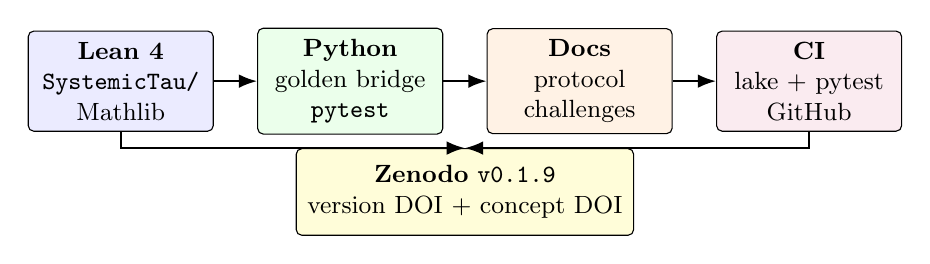
\begin{tikzpicture}[
  box/.style={draw, rounded corners=2pt, align=center, font=\small,
    minimum height=1.1cm, minimum width=2.35cm, inner sep=4pt},
  arr/.style={-{Latex}, thick}
]
  \node[box, fill=blue!8] (lean) {\textbf{Lean 4}\\\texttt{SystemicTau/}\\Mathlib};
  \node[box, fill=green!8, right=0.55cm of lean] (py) {\textbf{Python}\\golden bridge\\\texttt{pytest}};
  \node[box, fill=orange!10, right=0.55cm of py] (docs) {\textbf{Docs}\\protocol\\challenges};
  \node[box, fill=purple!8, right=0.55cm of docs] (ci) {\textbf{CI}\\lake + pytest\\GitHub};
  \node[box, fill=yellow!15, below=0.85cm of $(lean)!0.5!(ci)$] (zen)
    {\textbf{Zenodo} \texttt{v0.1.9}\\version DOI + concept DOI};
  \draw[arr] (lean) -- (py);
  \draw[arr] (py) -- (docs);
  \draw[arr] (docs) -- (ci);
  \draw[arr] (lean.south) |- ($(zen.north)+(-1.2,0)$) -- (zen.north);
  \draw[arr] (ci.south) |- ($(zen.north)+(1.2,0)$) -- (zen.north);
\end{tikzpicture}
\caption{Architecture of the monorepository: formal core, reference implementation,
documentation and scrutiny surfaces, continuous integration, and citable deposit.}
\label{fig:arch}
\end{figure}

\begin{figure}[ht]
\centering
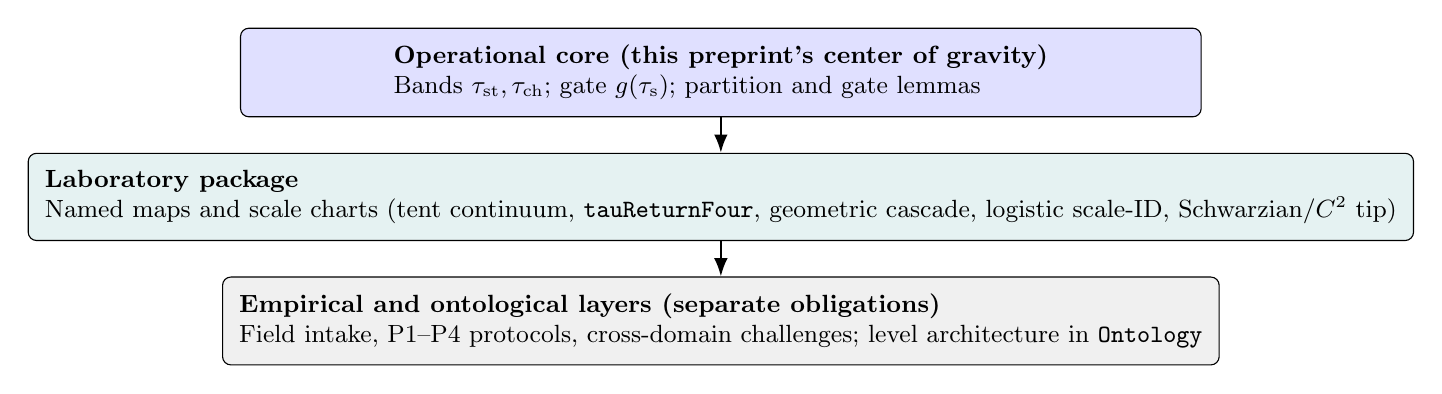
\begin{tikzpicture}[
  layer/.style={draw, rounded corners=3pt, align=left, font=\small,
    minimum width=12.2cm, inner sep=6pt},
  arr/.style={-{Latex}, thick}
]
  \node[layer, fill=blue!12] (op) {%
    \textbf{Operational core (this preprint's center of gravity)}\\
    Bands \(\taust,\tauch\); gate \(g(\taus)\); partition and gate lemmas};
  \node[layer, fill=teal!10, below=0.45cm of op] (lab) {%
    \textbf{Laboratory package}\\
    Named maps and scale charts (tent continuum, \texttt{tauReturnFour}, geometric cascade,
    logistic scale-ID, Schwarzian/\(C^2\) tip)};
  \node[layer, fill=gray!12, below=0.45cm of lab] (emp) {%
    \textbf{Empirical and ontological layers (separate obligations)}\\
    Field intake, P1--P4 protocols, cross-domain challenges; level architecture in \texttt{Ontology}};
  \draw[arr] (op) -- (lab);
  \draw[arr] (lab) -- (emp);
\end{tikzpicture}
\caption{Discourse layers. The checker verdict on the operational core and laboratory
package is kept distinct from field validation and ontological discussion.}
\label{fig:layers}
\end{figure}

%------------------------------------------------------------------
\section{Operational definitions}
%------------------------------------------------------------------

\subsection{Systemic Tau}

Consider a multivariate series and a sliding window of length \(W\) (default \(W=13\) in the reference core). On each window, Kendall-type rank correlations~\cite{kendall1938} are computed between variable pairs; \(\taus\) denotes the mean over those pairs. In Lean, the interface fixes rational types and an opaque symbol \texttt{kendallTau} for the combinatorial implementation. The remainder of the formalization reasons about \(\tau\in\mathbb{Q}\) without depending on a particular numerical backend.

\subsection{Regime bands}

The standard fixes two rational thresholds:
\begin{align}
  \taust &= \tfrac{1}{2}, \\
  \tauch &= \tfrac{41}{100}.
\end{align}

Regime classification on \(\tau\in\mathbb{Q}\) is summarized in Table~\ref{tab:bands} and Figure~\ref{fig:bands-gate}:
\begin{align}
  \mathrm{stable}
    &\quad\text{if }\tau \ge \taust, \\
  \mathrm{chaotic}
    &\quad\text{if }-\tauch < \tau < \tauch, \\
  \mathrm{antiSync}
    &\quad\text{if }\tau \le -\tauch, \\
  \mathrm{intermediate}
    &\quad\text{otherwise}.
\end{align}

\begin{table}[ht]
\centering
\caption{Operational regime bands (exact rationals), matching Lean \texttt{classify}.}
\label{tab:bands}
\begin{tabular}{@{}lll@{}}
\toprule
\textbf{Regime} & \textbf{Condition on \(\tau\)} & \textbf{Notes} \\
\midrule
stable & \(\tau \ge \taust\) & \(\taust = 1/2\) \\
intermediate & \(\tauch \le \tau < \taust\) & \(\tauch = 41/100\); residual of the cases below \\
chaotic & \(-\tauch < \tau < \tauch\) & open interval \\
antiSync & \(\tau \le -\tauch\) & left-closed ray \\
\bottomrule
\end{tabular}
\end{table}

On the nonnegative ray, an exhaustive trichotomy is proved: every \(\tau\ge 0\) falls into chaotic, intermediate, or stable, mutually exclusively under these definitions. The inequality \(\tauch<\taust\) is also established.

\subsection{Operational Feigenbaum constant}

A laboratory rational approximation
\[
  \deltaop
  = \frac{46692016091}{10000000000}
  \approx 4.6692016091
\]
is introduced. Explicitly: \(\deltaop\) is a \emph{fixed} rational approximation to classical \(\delta\), obtained by truncating the tabulated expansion to ten decimal places
(\(4.6692016091\ldots\mapsto 46692016091/10^{10}\)), following high-precision values in the period-doubling literature~\cite{feigenbaum1978,briggs1991}.
The numerator and denominator are encoded as naturals in Lean
(\texttt{feigenbaumDeltaNum}/\texttt{feigenbaumDeltaDen}); the package does not claim that this rational is the unique ``best'' approximant, only that it is the operational pin used throughout.
The gate prefactor is
\[
  p = \frac{\deltaop-1}{\deltaop}.
\]
Lean checks \(0<p<1\). The proximity quantity \(2/\deltaop\) satisfies
\[
  2/\deltaop > \tauch,
\]
with an explicit positive rational gap \(2/\deltaop - \tauch\) (order \(10^{-2}\)). That proximity motivates the chaotic band without imposing a closed identity \(\tauch=f(\delta)\).

%------------------------------------------------------------------
\section{The RECD gate}
%------------------------------------------------------------------

The reference gate law \(g:\mathbb{Q}\to\mathbb{Q}\) is defined piecewise by
\begin{equation}
\label{eq:gate}
  g(\tau) \;=\;
  \begin{cases}
    +1, &
      \text{if }\ \tau \ge \taust, \\[0.55em]
    \displaystyle
    p\cdot\frac{\tauch-|\tau|}{\tauch}, &
      \text{if }\ |\tau| < \tauch, \\[1.05em]
    -1, &
      \text{if }\ \tau \le -\tauch, \\[0.55em]
    0, &
      \text{otherwise}.
  \end{cases}
\end{equation}

\begin{figure}[H]
\centering
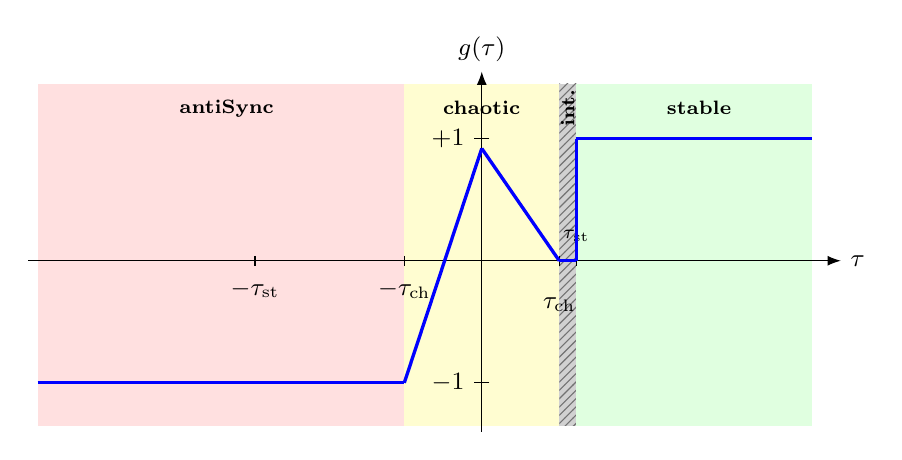
\begin{tikzpicture}[x=2.4cm,y=1.55cm,font=\small]
  % regions (patterns + fills: readable in greyscale print)
  \fill[red!12] (-2.35,-1.35) rectangle (-0.41,1.45);
  \fill[yellow!18] (-0.41,-1.35) rectangle (0.41,1.45);
  % positive intermediate: denser hatch so g=0 band survives greyscale
  \fill[black!18] (0.41,-1.35) rectangle (0.50,1.45);
  \fill[pattern=north east lines, pattern color=black!55]
    (0.41,-1.35) rectangle (0.50,1.45);
  \fill[green!12] (0.50,-1.35) rectangle (1.75,1.45);
  % axes
  \draw[-{Latex}] (-2.4,0) -- (1.9,0) node[right] {\(\tau\)};
  \draw[-{Latex}] (0,-1.4) -- (0,1.55) node[above] {\(g(\tau)\)};
  % ticks
  \foreach \x in {-1.2,-0.41,0.41,0.50} {
    \draw (\x,0.04) -- (\x,-0.04);
  }
  % staggered labels to avoid τch/τst collision
  \node[below] at (-1.2,-0.08) {\(-\taust\)};
  \node[below] at (-0.41,-0.08) {\(-\tauch\)};
  \node[below] at (0.41,-0.22) {\(\tauch\)};
  \node[above,font=\scriptsize] at (0.50,0.08) {\(\taust\)};
  \draw (0.04,1) -- (-0.04,1) node[left] {\(+1\)};
  \draw (0.04,-1) -- (-0.04,-1) node[left] {\(-1\)};
  % gate pieces (schematic continuous drawing)
  \draw[blue,very thick] (-2.35,-1) -- (-0.41,-1);
  \draw[blue,very thick] (-0.41,-1) -- (0,0.92);
  \draw[blue,very thick] (0,0.92) -- (0.41,0);
  \draw[blue,very thick] (0.41,0) -- (0.50,0);
  \draw[blue,very thick] (0.50,0) -- (0.50,1);
  \draw[blue,very thick] (0.50,1) -- (1.75,1);
  % region labels
  \node[font=\scriptsize\bfseries] at (-1.35,1.25) {antiSync};
  \node[font=\scriptsize\bfseries] at (0,1.25) {chaotic};
  \node[font=\scriptsize\bfseries] at (0.455,1.25) {\rotatebox{90}{int.}};
  \node[font=\scriptsize\bfseries] at (1.15,1.25) {stable};
\end{tikzpicture}
\caption{Schematic of operational bands on the \(\tau\)-axis and the piecewise gate
\(g(\tau)\) from Equation~\eqref{eq:gate}. The narrow hatched strip is the positive
intermediate band where \(g=0\). Note the asymmetric treatment of the anti-synchronous
ray (\(g=-1\)) relative to that strip.}
\label{fig:bands-gate}
\end{figure}

Formal properties included in the core (and accepted by Lean) include:

\begin{itemize}[leftmargin=1.2em]
  \item \textbf{Closed form on \([0,\tauch)\).}
        Equation~\eqref{eq:gate} reduces to
        \(g(\tau)=p\,(\tauch-\tau)/\tauch\).
  \item \textbf{Antitonicity (non-increasing on the positive chaotic ray).}
        If \(0\le a\le b<\tauch\), then \(g(b)\le g(a)\).
        As \(\tau\) grows toward the band edge, the nonnegative gate value does not increase.
        Since \(g\ge 0\) on that ray, the same holds for \(|g|\): magnitude is non-increasing in \(\tau\).
  \item \textbf{Boundedness.}
        From the piecewise law: \(|g(\tau)|\le 1\) for every regime.
        Stable and antiSync saturate at \(\pm 1\);
        the chaotic piece is \(p\in(0,1)\) times a factor in \((0,1]\), hence strictly below \(1\)
        except at the origin, where \(g(0)=p\).
  \item \textbf{Exact zero on the positive intermediate band.}
        \(\tauch\le\tau<\taust\) implies \(g(\tau)=0\).
  \item \textbf{Edge samples and regime links.}
        \(g(3/4)=1\), \(g(-3/4)=-1\), \(g(45/100)=0\), \(g(0)=p\);
        \(g(\tau)=1\) for all \(\tau\ge\taust\);
        \(g(\tau)=-1\) for all \(\tau\le-\tauch\).
        Local evenness holds inside the open chaotic band
        (\(g(-\tau)=g(\tau)\) when \(|\tau|<\tauch\)),
        but the law is \emph{not} globally even: the anti-synchronous ray opens at \(-1\)
        while the positive intermediate band stays closed at \(0\).
  \item \textbf{Piecewise character.}
        On \(\mathbb{Q}\), \(g\) is a finite piecewise-rational function of \(\tau\) and
        \(|\tau|\). Each piece is affine in \(\tau\) (or constant). Jumps appear only at
        the band boundaries encoded in Equation~\eqref{eq:gate}
        (notably \(\tau=\pm\tauch\) and \(\tau=\taust\)).
\end{itemize}

\paragraph{Numerical illustration.}
Table~\ref{tab:gate-samples} lists a short synthetic walk of \(\taus\) values
and the corresponding gate signal under Equation~\eqref{eq:gate}
(with \(p=(\deltaop-1)/\deltaop\)). Figure~\ref{fig:synthetic} plots the same walk.

\begin{table}[ht]
\centering
\caption{Synthetic \(\taus\) walk and gate response (rational arithmetic).}
\label{tab:gate-samples}
\begin{tabular}{@{}cccc@{}}
\toprule
\(t\) & \(\taus\) & Regime & \(g(\taus)\) \\
\midrule
1 & \(0.55\) & stable & \(+1\) \\
2 & \(0.48\) & intermediate & \(0\) \\
3 & \(0.30\) & chaotic & \(p\cdot(0.41-0.30)/0.41\) \\
4 & \(0.10\) & chaotic & \(p\cdot(0.41-0.10)/0.41\) \\
5 & \(0.00\) & chaotic & \(p\) \\
6 & \(-0.20\) & chaotic & \(p\cdot(0.41-0.20)/0.41\) \\
7 & \(-0.45\) & antiSync & \(-1\) \\
8 & \(0.60\) & stable & \(+1\) \\
\bottomrule
\end{tabular}
\end{table}

\begin{figure}[H]
\centering
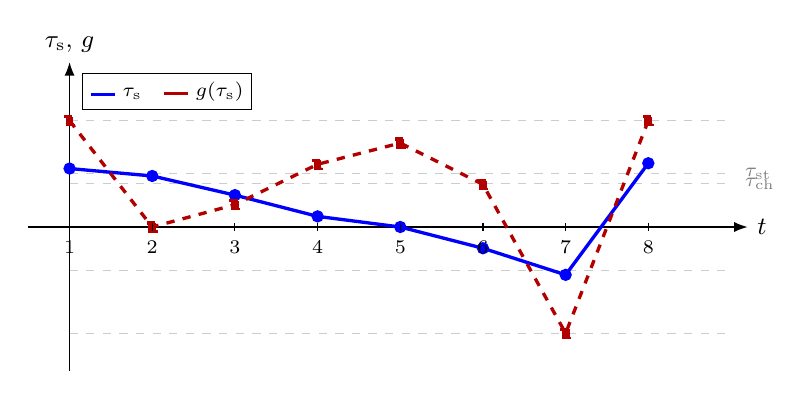
\begin{tikzpicture}[x=1.05cm,y=1.35cm,font=\small]
  % axes
  \draw[-{Latex}] (0.5,0) -- (9.2,0) node[right] {\(t\)};
  \draw[-{Latex}] (1,-1.35) -- (1,1.55) node[above] {\(\taus,\,g\)};
  % horizontal guides
  \draw[gray!40,dashed] (1,1) -- (9,1);
  \draw[gray!40,dashed] (1,-1) -- (9,-1);
  \draw[gray!40,dashed] (1,0.5) -- (9,0.5);
  \draw[gray!40,dashed] (1,0.41) -- (9,0.41);
  \draw[gray!40,dashed] (1,-0.41) -- (9,-0.41);
  \node[font=\scriptsize,gray,anchor=west] at (9.05,0.50) {\(\taust\)};
  \node[font=\scriptsize,gray,anchor=west] at (9.05,0.41) {\(\tauch\)};
  % tau series (approx values)
  \draw[blue,very thick,mark=*,mark size=1.6pt]
    plot coordinates {
      (1,0.55) (2,0.48) (3,0.30) (4,0.10)
      (5,0.00) (6,-0.20) (7,-0.45) (8,0.60)
    };
  % gate series (schematic: p≈0.786)
  \draw[red!70!black,very thick,dashed,mark=square*,mark size=1.4pt]
    plot coordinates {
      (1,1.00) (2,0.00) (3,0.21) (4,0.59)
      (5,0.79) (6,0.40) (7,-1.00) (8,1.00)
    };
  % legend box
  \node[draw,fill=white,inner sep=3pt,anchor=north west,font=\scriptsize] at (1.15,1.45) {%
    \textcolor{blue}{\rule{1.1em}{1.2pt}} \(\taus\)\quad
    \textcolor{red!70!black}{\rule[0.4pt]{1.1em}{1.0pt}} \(g(\taus)\)};
  \foreach \t in {1,2,3,4,5,6,7,8} {
    \draw (\t,0.04) -- (\t,-0.04) node[below,font=\scriptsize] {\t};
  }
\end{tikzpicture}
\caption{Synthetic eight-step walk of \(\taus\) (solid) and the RECD gate
\(g(\taus)\) (dashed). Intermediate positive \(\taus\) keeps the gate closed;
antiSync opens it at \(-1\); high coherence saturates at \(+1\).}
\label{fig:synthetic}
\end{figure}

%------------------------------------------------------------------
\section{Feigenbaum laboratory package}
%------------------------------------------------------------------

Beyond the gate, the repository develops a package of \emph{laboratory constructions}.
They connect the language of \(\taus\) to unimodal dynamics and the period-doubling
cascade~\cite{feigenbaum1978,deMellovanStrien,lyubich1999}.
The constructions live in dedicated Lean modules and build together with the core.

\subsection{Reduction and return maps}

The first laboratory layer asks a concrete question: which maps may stand in, inside the checker, for a return of a coherence-like coordinate?
The reduction module answers with named objects rather than prose: realizers of functional pairs, a laboratory continuum based on the tent map, and a continuous non-tent return \texttt{tauReturnFour} (logistically conjugate on a coherence interval).
A composite package then pairs that return with a refined \texttt{FeigenbaumUniversal} object (operational \(\delta\)-band and quadratic tip).
The scientific claim at this layer is modest: the bridge exists as citable, verified constructions---not as informal narrative.

\subsection{Analytic cascade and topology}

Once return maps are available, the package freezes a geometric parameter cascade whose exact ratio is \(\deltaop\).
Scaling ratios of that cascade are proved equal to \(\deltaop\).
Within the formalism, the classical \(\varepsilon\)--\(N\) notion of cascade limit is shown equivalent to a \texttt{Tendsto}-style convergence statement, so topological language and sequential bookkeeping stay aligned.
Honesty blocks include toy cascades that do \emph{not} approach \(\deltaop\); the checker therefore distinguishes models that satisfy the scaling ratio from those that do not.

\subsection{Logistic scale identification}

The logistic chart is the usual first contact for readers of one-dimensional dynamics.
A dedicated module anchors a parameter sequence at landmarks \(r_0=2\), \(r_1=3\) and proves that this sequence shares scale (ratios) with the geometric cascade above.
It is a laboratory scale identification between two parameter charts, expressed in Lean: not a claim that field \(\taus\) is logistic, but a shared ruler for later comparison.

\subsection{Quadratic tip and Schwarzian}

Classical route-to-chaos arguments rely on tip geometry and Schwarzian control~\cite{singer1978}.
On the logistic map, the package formalizes derivatives, a quadratic tip with \(f''\ne 0\) at the critical point, the Schwarzian inequality off the critical point, and a \texttt{FeigenbaumUniversalC2} assembly of operational band and tip.
The point for a non-Lean reader is simple: \(C^2\)/Schwarzian vocabulary lives inside the accepted artifact, ready for attack or extension, without being smuggled into the operational core of Equation~\eqref{eq:gate}.

\subsection{Module inventory}

\begin{table}[H]
\centering
\caption{Lean modules under \texttt{SystemicTau/} (v0.1.9).}
\label{tab:modules}
\begin{tabular}{@{}llclp{5.4cm}@{}}
\toprule
\textbf{Module} & \textbf{Lines} & \textbf{Status} & \textbf{Content} \\
\midrule
\texttt{Basic} & \(\sim\)50 & Core & Types, \(\deltaop\), window, regimes \\
\texttt{Thresholds} & \(\sim\)240 & Core & Bands, trichotomy, simple \(f(\delta)\) non-IDs \\
\texttt{ThresholdFromDelta} & \(\sim\)500 & Core & Unique inverse-scale \(f(\delta)=c/\delta\) \\
\texttt{RECD} & \(\sim\)240 & Core & Gate \(g\), antitonicity, samples \\
\texttt{FeigenbaumReduction} & \(\sim\)1050 & Lab & Returns, composite package \\
\texttt{FeigenbaumAnalytic} & \(\sim\)440 & Lab & Geometric cascade, \(\varepsilon\)--\(N\) \\
\texttt{FeigenbaumTendsto} & \(\sim\)280 & Lab & Equivalence with \texttt{Tendsto} \\
\texttt{FeigenbaumLogistic} & \(\sim\)250 & Lab & Logistic scale identification \\
\texttt{FeigenbaumSchwarzian} & \(\sim\)200 & Lab & Quadratic tip, Schwarzian \\
\texttt{Ontology} & \(\sim\)70 & Spec & L0--L3 levels; stratified claims \\
\bottomrule
\end{tabular}
\end{table}

The \texttt{SystemicTau/} directory of version 0.1.9 builds end to end in Lean~4.14 with Mathlib~\texttt{v4.14.0}~\cite{lean4,mathlib}.

\subsection{Formal status summary}

Table~\ref{tab:status} states, in one place, what the checker has accepted, what is packaged as named laboratory construction, and what remains an open research obligation. This table is part of the scientific claim of the release.

\begin{table}[H]
\centering
\caption{Formal status of the v0.1.9 package under \texttt{SystemicTau/}.}
\label{tab:status}
\begin{tabularx}{\textwidth}{@{}>{\bfseries}p{2.8cm}X@{}}
\toprule
Proved (core) &
\begin{minipage}[t]{\linewidth}\raggedright\smallskip
Band ordering \(\tauch<\taust\); nonnegative trichotomy of \texttt{classify};
gate formula on \([0,\tauch)\); antitonicity of \(g\) on that half-band;
positive intermediate closure \(g=0\); canonical samples;
gate prefactor bounds \(0<p<1\); gap \(2/\deltaop>\tauch\);
finite simple closed forms \(\neq\tauch\) (ten rational candidates);
unique inverse-scale bridge \(f(\delta)=c/\delta\) with
\(f(\deltaop)=\tauch\) and \(\taust=1/2\) (class-conditional uniqueness).
\smallskip\end{minipage} \\
\midrule
Proved (lab lemmas) &
\begin{minipage}[t]{\linewidth}\raggedright\smallskip
Geometric cascade ratios equal to \(\deltaop\);
\(\varepsilon\)--\(N\) \(\Leftrightarrow\) \texttt{Tendsto} bookkeeping;
logistic scale identification with the geometric chart;
Schwarzian \(\le 0\) off the critical point (formal derivatives);
quadratic tip package; zero \texttt{sorry} and zero author research \texttt{axiom}
under \texttt{SystemicTau/}.
\smallskip\end{minipage} \\
\midrule
Laboratory constructions (named, accepted) &
\begin{minipage}[t]{\linewidth}\raggedright\smallskip
\texttt{lookupTent} realizers; tent continuum return;
non-tent continuum return \texttt{tauReturnFour};
refined \texttt{FeigenbaumUniversal} / \texttt{FeigenbaumUniversalC2};
composite laboratory packages built from the above.
\smallskip\end{minipage} \\
\midrule
Explicitly open &
\begin{minipage}[t]{\linewidth}\raggedright\smallskip
Termwise superstable logistic roots;
Mathlib \(C^2\)-open renormalization / fixed-point universality~\cite{lyubich1999};
field-derived continuum return of \(\taus\) (not a cited lab map);
classical free-\(c\) derivation of \(\tauch\) from pure Feigenbaum
(naive \(f=2/\delta\) fails machine-checked);
multi-site empirical P1/P4 discharge.
\smallskip\end{minipage} \\
\bottomrule
\end{tabularx}
\end{table}

%------------------------------------------------------------------
\section{Python reference core and open science}
%------------------------------------------------------------------

The monorepository is not limited to the proof assistant. It includes a Python core with golden rationals aligned to Lean (\texttt{python/core/golden.py}) and \texttt{pytest} tests; synthetic fixtures, noise and anti-synchrony protocols, and a first-return twin for numerical exploration; data paths and notebooks for field series (e.g., \emph{Aedes}) and synthetic cross-domain kits; continuous integration (\texttt{lake build} + \texttt{pytest}) on GitHub Actions; and release \texttt{v0.1.9} with version DOI
\href{https://doi.org/10.5281/zenodo.21536462}{10.5281/zenodo.21536462}
and concept DOI
\href{https://doi.org/10.5281/zenodo.21516059}{10.5281/zenodo.21516059},
under MIT license with citation metadata (\texttt{CITATION.cff}).

The Lean--Python combination is deliberate. Lean certifies the criterion; Python makes it operable in data-analysis workflows. Companion materials include a broader narrative synthesis of the paradigm~\cite{padilla2026magna} and the production package \texttt{systemictau} on PyPI.

%------------------------------------------------------------------
\section{How verification is reproduced}
%------------------------------------------------------------------

In an environment with \texttt{elan} and Lean~4.14:

\begin{verbatim}
git clone https://github.com/johelpadilla/systemic-tau-formal.git
cd systemic-tau-formal/lean
lake exe cache get   # recommended
lake build
cd ../python
pip install -e ".[dev]"
pytest -q
\end{verbatim}

A successful \texttt{SystemicTau} build constitutes the public checker verdict on the formal core described here. Generated \texttt{.olean} artifacts document, in the sense of formal proof engineering, that the package was accepted by the kernel.

%------------------------------------------------------------------
\section{Scrutiny program}
%------------------------------------------------------------------

The standard is accompanied by an open critique program documented in the repository:

\begin{itemize}[leftmargin=1.2em]
  \item \textbf{Falsifiable predictions and experimental protocol} for early-warning style claims in the \(\taus\)/RECD setting~\cite{scheffer2009,dakos2012,boettiger2013}.
  \item \textbf{Challenge C1} --- systematic false early warnings: stress the gate under controlled noise and anti-synchrony (P3/P4 style attacks).
  \item \textbf{Challenge C2} --- new mathematical relations: propose and formalize relations beyond the finite non-identities already recorded for \(\tauch\) versus simple functions of \(\delta\).
  \item \textbf{Challenge C3} --- domain transfer: carry the operational criterion to licensed field series outside the synthetic kits (finance, EEG, grid, or other domains).
  \item \textbf{Stress-Test 2026} --- an open invitation to host structured attacks on the criterion and its laboratory bridges.
  \item \textbf{Level architecture} --- ontological specification kept in module \texttt{Ontology}, so that philosophical conversation is not confused with the checker's acceptance of \(g\) and the bands.
\end{itemize}

Attack metrics already instrumented in the reference code include agreement under additive noise at fixed \(\rho\) (P3), anti-synchrony response (P4), and a P1 endpoint scorer scaffold awaiting pre-registered observation times. The message to the community is invitation: the paradigm can be inspected, cloned, and attacked under written rules.

%------------------------------------------------------------------
\section{Discussion}
%------------------------------------------------------------------

\subsection{The value of a small, hard criterion}

In complex systems it is tempting to multiply indicators. This work inverts the priority: a small object---rational bands and a piecewise gate---receives the treatment of a formal standard. The strength of the approach is auditability. A reviewer can point to the exact line of a definition or lemma.

\subsection{Laboratory constructions as a public language}

Laboratory constructions are not decorative illustrations of a prose story. They are the \emph{shared vocabulary} in which the paradigm can speak to dynamics without smuggling field claims into the operational core. Each construction is named, cited from Lean identifiers, and accepted by the same checker as the gate. A critic can therefore accept the operational standard while rejecting a particular laboratory map---or the reverse---without collapsing the whole package. That separability is what makes the laboratory language public rather than private metaphor.

\subsection{Related work and positioning}

Period-doubling universality has a mature analytic literature~\cite{feigenbaum1978,briggs1991,deMellovanStrien,lyubich1999,singer1978}.
Formal mathematics ecosystems (Lean/Mathlib, Isabelle, Coq) increasingly host dynamical and analysis libraries~\cite{lean4,mathlib}, though full machine-checked proofs of classical Feigenbaum universality remain an open frontier rather than a commodity theorem.
Early-warning research provides both positive methods~\cite{scheffer2009,dakos2012} and critical caution about pattern-to-prediction overclaim~\cite{boettiger2013,boettiger2012}.
The present artifact sits between these literatures: it does not re-prove classical universality, and it does not market \(\taus\) as an automatic field detector. It freezes a small operational core that a checker accepts, and it packages laboratory maps as named, attackable objects. Prior narrative synthesis of the broader paradigm appears in~\cite{padilla2026magna}; the formal monorepository is the citable operational pin~\cite{systemic-tau-formal}.

\subsection{Open science as part of the claim}

DOIs, continuous integration, and the public repository are not administrative annexes. They form part of what the paradigm says of itself: that it aspires to be shared infrastructure. A standard that cannot be cloned is not a standard; it is an announcement.

\subsection{Layers of discourse}

The monorepository organizes work into layers that are read differently (Figure~\ref{fig:layers}). The operational core and laboratory constructions are the object of this preprint. Field empirical validation and ontological readings live in the same ecosystem under their own obligations. That separation is itself a thesis: not to conflate the checker's verdict with the verdict of data or of metaphysics.

This preprint does not claim to settle the classical Feigenbaum universality theorem, nor to derive \(\taus\) dynamics from first principles of a physical field. It offers a checkable operational core and a laboratory language in which such questions can be attacked.

%------------------------------------------------------------------
\section{Conclusion}
%------------------------------------------------------------------

We have presented \texttt{systemic-tau-formal}~v0.1.9 as a Lean-accepted operational standard for Systemic Tau and RECD, together with a laboratory construction package and an open scrutiny program. The repository offers:

\begin{enumerate}[leftmargin=1.4em]
  \item rational definitions of \(\taust\), \(\tauch\), and \(g(\taus)\);
  \item classification, trichotomy, and gate-behavior lemmas;
  \item a Feigenbaum-line laboratory construction package accepted by Lean;
  \item an aligned Python core, continuous integration, and a citable deposit.
\end{enumerate}

To others, the artifact says that this paradigm can already be inspected from outside: there is a written criterion, a checker that accepts it, and an open door to scrutiny. That is the contribution recorded here.

%------------------------------------------------------------------
\section*{Data and code availability}
%------------------------------------------------------------------

Source code and releases: \url{https://github.com/johelpadilla/systemic-tau-formal}.\\
Software version associated with this text: \texttt{v0.1.9}.\\
Preprint document version: \texttt{0.1.9-r1} (2026-07-24).\\
Preprint DOI: \href{https://doi.org/10.5281/zenodo.21536465}{10.5281/zenodo.21536465}.\\
Software version DOI: \href{https://doi.org/10.5281/zenodo.21536462}{10.5281/zenodo.21536462}.\\
Software concept DOI: \href{https://doi.org/10.5281/zenodo.21516059}{10.5281/zenodo.21516059}.\\
Related production package on PyPI: \texttt{systemictau}.\\[0.4em]
Minimal verification:
\begin{verbatim}
cd lean && lake build && cd ../python && pytest -q
\end{verbatim}

%------------------------------------------------------------------
\section*{Acknowledgments}
%------------------------------------------------------------------

The author acknowledges the Lean and Mathlib communities for the formal verification infrastructure that makes standards of this kind possible, and those who will take part in open scrutiny of the repository.

%------------------------------------------------------------------
\appendix
\section{Release note relative to v0.1.8}
\label{app:changelog}

Version 0.1.9 is a formal-track pin of the threshold-bridge pack on top of the
v0.1.8 laboratory construction release:

\begin{itemize}[leftmargin=1.2em]
  \item Module \texttt{ThresholdFromDelta}: unique operational
        \(f(\delta)=c/\delta\) with \(c_\star=\tauch\cdot\deltaop\).
  \item Extended \texttt{failedSimpleCandidates} (ten rational non-identities).
  \item Ontology L0--L3 registry and \texttt{stratifiedFour} bookkeeping.
  \item Still zero \texttt{sorry} and zero author research \texttt{axiom}.
  \item Retained from v0.1.8: non-tent return, logistic scale-ID, Schwarzian pack.
\end{itemize}

\section{Expanded module map}
\label{app:modules}

Table~\ref{tab:modules-detail} expands the inventory of Section~5 for readers who want a denser map of the Lean surface. Line counts are approximate at the v0.1.9 pin.

\begin{table}[H]
\centering
\caption{Expanded \texttt{SystemicTau/} module map (v0.1.9).}
\label{tab:modules-detail}
\begin{tabularx}{\textwidth}{@{}l>{\raggedright\arraybackslash}p{1.4cm}X@{}}
\toprule
\textbf{Module} & \textbf{Status} & \textbf{Primary surface} \\
\midrule
\texttt{Basic} & Core &
  Rational types; \(\deltaop\) numerator/denominator;
  window default; regime enum; gate prefactor \(p\). \\
\texttt{Thresholds} & Core &
  \(\taust,\tauch\); \texttt{classify}; nonnegative trichotomy;
  band ordering; proximity gap \(2/\deltaop>\tauch\);
  extended simple-form non-identities. \\
\texttt{ThresholdFromDelta} & Core &
  Inverse-scale class; unique \(c_\star\); antitonicity of \(f\);
  pair recovery at \(\deltaop\); gate/partition compatibility;
  honesty block for pure \(2/\delta\). \\
\texttt{RECD} & Core &
  \texttt{gate}; chaos closed form; antitonicity;
  intermediate zero; stable/antiSync saturations; samples;
  local evenness on the open chaotic band; tick units. \\
\texttt{FeigenbaumReduction} & Lab &
  Tent realizers; continuum returns; \texttt{tauReturnFour};
  unimodal/hump lemmas; composite \texttt{FeigenbaumUniversal}. \\
\texttt{FeigenbaumAnalytic} & Lab &
  Geometric cascade with ratio \(\deltaop\);
  scaling-ratio theorems; honesty (non-\(\delta\)) blocks. \\
\texttt{FeigenbaumTendsto} & Lab &
  \(\varepsilon\)--\(N\) \(\Leftrightarrow\) \texttt{Tendsto} bookkeeping;
  real casts of cascade quantities. \\
\texttt{FeigenbaumLogistic} & Lab &
  Landmarks \(r_0=2\), \(r_1=3\); scale identification with the geometric chart. \\
\texttt{FeigenbaumSchwarzian} & Lab &
  Formal derivatives; quadratic tip; Schwarzian \(\le 0\) off critical point;
  \texttt{FeigenbaumUniversalC2}. \\
\texttt{Ontology} & Spec &
  L0--L3 levels; well-sited claims; \texttt{stratifiedFour}
  (discourse layer; not an operational theorem). \\
\bottomrule
\end{tabularx}
\end{table}

\clearpage
%------------------------------------------------------------------
\begin{thebibliography}{99}

\bibitem{feigenbaum1978}
M.~J. Feigenbaum.
\newblock Quantitative universality for a class of nonlinear transformations.
\newblock \emph{Journal of Statistical Physics}, 19(1):25--52, 1978.

\bibitem{briggs1991}
K.~Briggs.
\newblock A precise calculation of the Feigenbaum constants.
\newblock \emph{Mathematics of Computation}, 57(195):435--439, 1991.

\bibitem{deMellovanStrien}
W.~de~Melo and S.~van~Strien.
\newblock \emph{One-Dimensional Dynamics}.
\newblock Springer, 1993.

\bibitem{lyubich1999}
M.~Lyubich.
\newblock Feigenbaum--Coullet--Tresser universality and Milnor's hairiness conjecture.
\newblock \emph{Annals of Mathematics}, 149(2):319--420, 1999.

\bibitem{singer1978}
D.~Singer.
\newblock Stable orbits and bifurcation of maps of the interval.
\newblock \emph{SIAM Journal on Applied Mathematics}, 35(2):260--267, 1978.

\bibitem{lean4}
L.~de~Moura and S.~Ullrich.
\newblock The Lean~4 theorem prover and programming language.
\newblock In \emph{Automated Deduction -- CADE 28}, pages 625--630. Springer, 2021.

\bibitem{mathlib}
The mathlib Community.
\newblock The Lean mathematical library.
\newblock In \emph{Proceedings of the 9th ACM SIGPLAN International Conference
  on Certified Programs and Proofs (CPP)}, pages 367--381, 2020.

\bibitem{kendall1938}
M.~G. Kendall.
\newblock A new measure of rank correlation.
\newblock \emph{Biometrika}, 30(1/2):81--93, 1938.

\bibitem{scheffer2009}
M.~Scheffer et al.
\newblock Early-warning signals for critical transitions.
\newblock \emph{Nature}, 461:53--59, 2009.

\bibitem{dakos2012}
V.~Dakos et al.
\newblock Methods for detecting early warnings of critical transitions in time
  series illustrated using simulated ecological data.
\newblock \emph{PLOS ONE}, 7(7):e41010, 2012.

\bibitem{boettiger2013}
C.~Boettiger and A.~Hastings.
\newblock Tipping points: From patterns to predictions.
\newblock \emph{Nature}, 493:157--158, 2013.

\bibitem{boettiger2012}
C.~Boettiger and A.~Hastings.
\newblock Early warning signals and the prosecutor's fallacy.
\newblock \emph{Proceedings of the Royal Society B}, 279:4734--4739, 2012.

\bibitem{padilla2026magna}
J.~Padilla-Villanueva.
\newblock Síntesis Magna del Tau Sistémico.
\newblock Zenodo, 2026.
\newblock \href{https://doi.org/10.5281/zenodo.20576241}{doi:10.5281/zenodo.20576241}.

\bibitem{systemic-tau-formal}
J.~Padilla-Villanueva.
\newblock systemic-tau-formal: Machine-verifiable Systemic Tau (\(\taus\)) and RECD (v0.1.9).
\newblock Zenodo, 2026.
\newblock \href{https://doi.org/10.5281/zenodo.21536462}{doi:10.5281/zenodo.21536462}.

\bibitem{preprint-standard-formal}
J.~Padilla-Villanueva.
\newblock A machine-checkable operational standard for Systemic Tau \(\taus\) and the Discrete Extramental Clock (RECD) (preprint 0.1.9-r1).
\newblock Zenodo, 2026.
\newblock \href{https://doi.org/10.5281/zenodo.21536465}{doi:10.5281/zenodo.21536465}.

\end{thebibliography}

\end{document}
